%Copyright 2019 Christopher M. Jermaine (cmj4@rice.edu) and Risa B. Myers (rbm2@rice.edu)
%
%Licensed under the Apache License, Version 2.0 (the "License");
%you may not use this file except in compliance with the License.
%You may obtain a copy of the License at
%
%    https://www.apache.org/licenses/LICENSE-2.0
%
%Unless required by applicable law or agreed to in writing, software
%distributed under the License is distributed on an "AS IS" BASIS,
%WITHOUT WARRANTIES OR CONDITIONS OF ANY KIND, either express or implied.
%See the License for the specific language governing permissions and
%limitations under the License.
%===============================================================
\documentclass[aspectratio=169]{beamer}
\mode<presentation> 
{
\usetheme[noshadow, minimal,numbers,riceb,nonav]{Rice}
\usefonttheme[onlymath]{serif}
\setbeamercovered{transparent}
}
\useinnertheme{rectangles}

\usepackage[english]{babel}

\usepackage{amsmath}
\usepackage{mathptmx}
\usepackage{helvet}
\usepackage{courier}
\usepackage[T1]{fontenc}
\usepackage{trajan}
\usepackage{ textcomp }
\usepackage{listings}

\newenvironment{noindentitemize}
{ \begin{itemize}
 \setlength{\itemsep}{1.5ex}
  \setlength{\parsep}{0pt}   
  \setlength{\parskip}{0pt}
 \addtolength{\leftskip}{-2em}
 }
{ \end{itemize} }

\newenvironment{noindentitemize2}
{ \begin{itemize}
  \setlength{\itemsep}{0ex}
  \setlength{\parskip}{0pt}
  \setlength{\parsep}{0pt}   
  \addtolength{\leftskip}{-2em}  }
{ \end{itemize} }

\lstnewenvironment{SQL}
  {\lstset{
        aboveskip=5pt,
        belowskip=5pt,
        escapechar=!,
        mathescape=true,
        upquote=true,
        language=SQL,
        basicstyle=\linespread{0.94}\ttfamily\footnotesize,
        morekeywords={WHILE, DO, END},
        deletekeywords={VALUE, PRIOR},
        showstringspaces=true}
        \vspace{0pt}%
        \noindent\minipage{0.47\textwidth}}
  {\endminipage\vspace{0pt}}
  
\newcommand{\LIKES}{\textrm{LIKES}} 
\newcommand{\FREQUENTS}{\textrm{FREQUENTS}} 
\newcommand{\SERVES}{\textrm{SERVES}} 
\newcommand{\CAFE}{\textrm{CAFE}} 
\newcommand{\COFFEE}{\textrm{COFFEE}} 
\newcommand{\DRINKER}{\textrm{DRINKER}} 
\newcommand{\ALLPEEPS}{\textrm{ALLPEEPS}} 
\newcommand{\ALLCOMBOS}{\textrm{ALLCOMBOS}} 


\setbeamerfont{block body}{size=\tiny}
%\setbeamerfont{block title example}{size=\Huge}

%===============================================================%

\title[]
{Tools \& Models for Data Science}

\subtitle{Outliers}

\author[]{Chris Jermaine \& Risa Myers}
\institute
{
  Rice University 
}

\date[]{}

\subject{Beamer}

\begin{document}

\begin{frame}
 \titlepage
\end{frame}

%***********************************************************
\begin{frame}{What Are Outliers In Data Science?}

\begin{itemize}
	\item Data points that are unlike the other points, unexpected, or unusual in some way
	\begin{itemize}
		\item Weather data set: low of -12$^{\circ}$C degrees in Houston
		\item Blood pressure > 300 mmHg
		\item Drug price change from \$13.50/pill to \$750/pill
	\end{itemize}
\end{itemize}

% regularly see BP in low 200's during surgery

% Daraprim approved in 1953
% used for treating parasite infections
% CEO of Turing Pharmaceuticals - just sentenced to 7 years in jail
\end{frame}
%***********************************************************
\begin{frame}{Outlier Pic: 1}

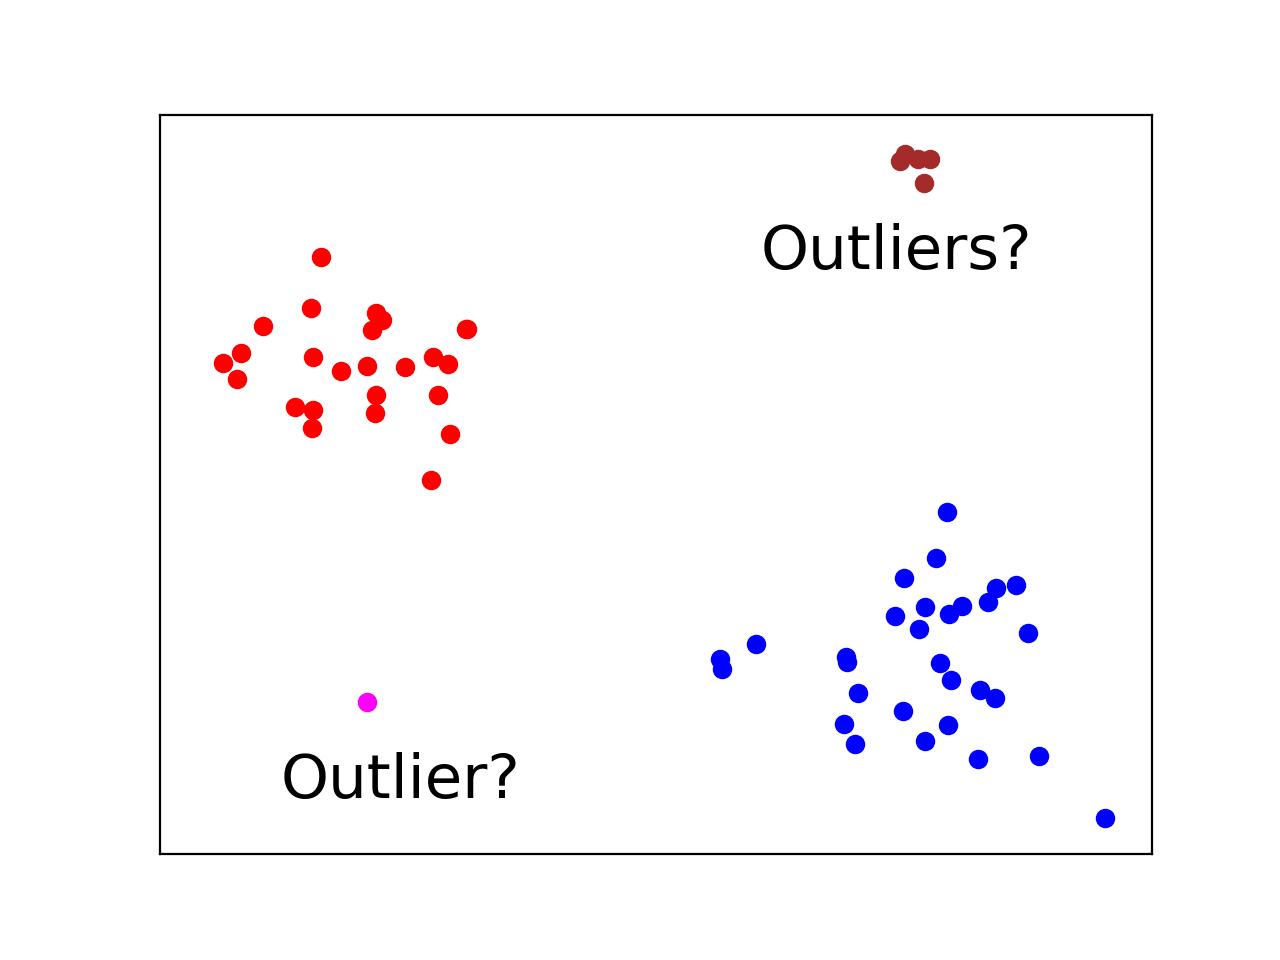
\includegraphics[width=.75\textwidth]{lectOutliers/2dOutliers.png}

\end{frame}
%***********************************************************
\begin{frame}{Outlier Pic: 2}

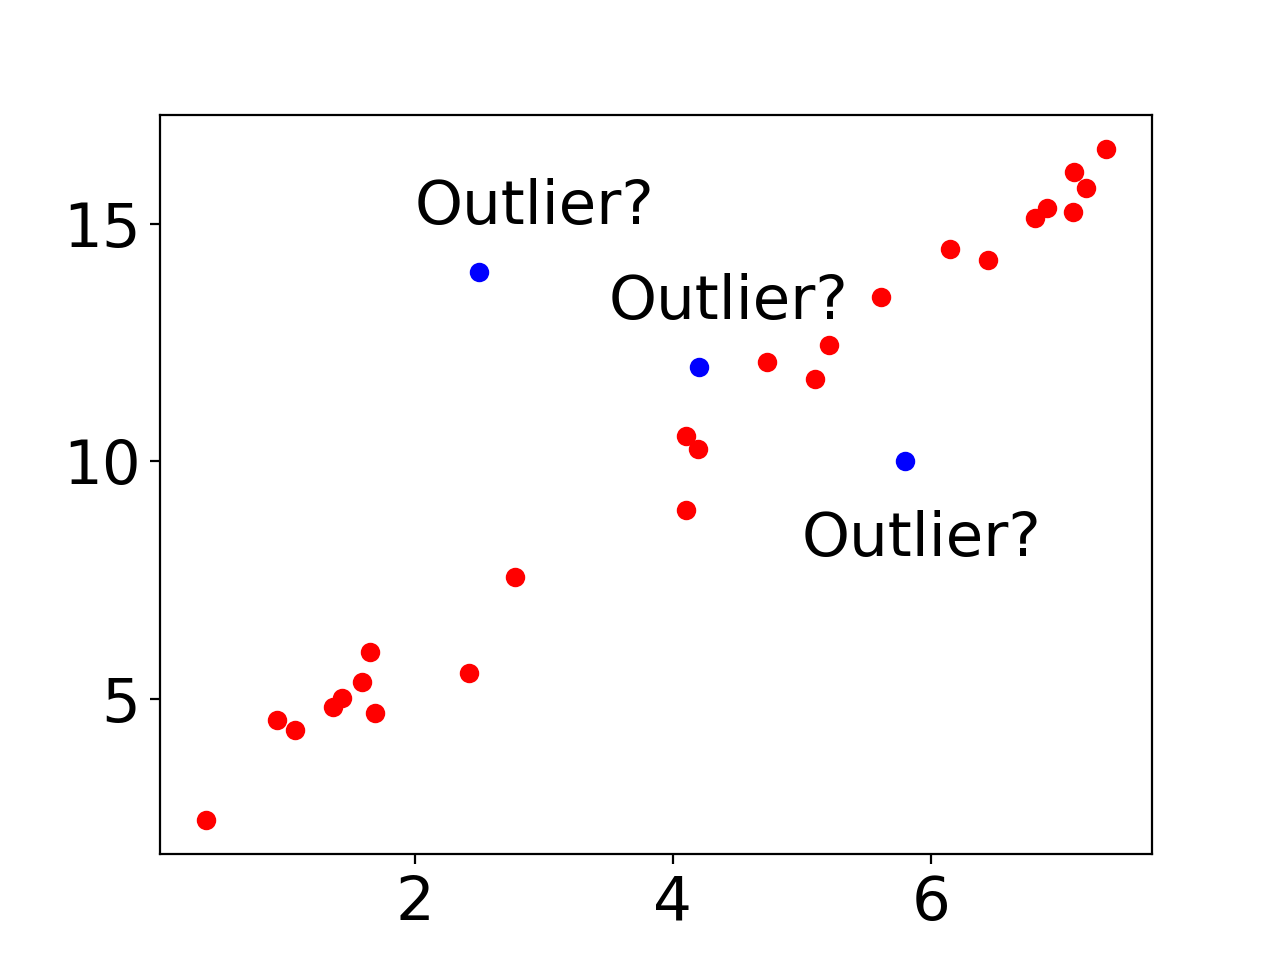
\includegraphics[width=0.7\textwidth]{lectOutliers/outlier_pic_2.png}

\end{frame}
%***********************************************************
\begin{frame}{Outliers Not Same As Unusual Data}

\begin{itemize}
	\item Low of 12$^{\circ}$C degrees in Houston unusual, probably not an outlier
	\item Low of -12$^{\circ}$C in Chicago (a bit) unusual, probably not an outlier
	\item It's the combination of Houston, -12$^{\circ}$C that makes this difficult to believe
\end{itemize}

\end{frame}
%***********************************************************
\begin{frame}{Why Look For Outliers?}

\begin{itemize}
	\item Classically, two reasons:
        \begin{enumerate}
		\item Classically, to remove them from data...
        \end{enumerate}
        \begin{itemize}
		\item ...because outliers can hurt learning process
        \end{itemize}
\end{itemize}

\end{frame}
%***********************************************************
\begin{frame}{Why Throw Out Data?}

\begin{itemize}
        \item It messes up the model
        \item Garbage in, garbage out
        \item Huge impact on least squares
        \begin{itemize}
        	\item Most common loss / error model
	\item Outliers have a magnified effect
        \end{itemize}
\end{itemize}
\begin {table}[!htbp]
\begin{center}
\begin{tabular}{|r|r|}
\hline
distance & distance$^2$ \\ \hline
1 & 1 \\ \hline
2 & 4  \\ \hline
-3 & 9 \\ \hline
-4 & 16 \\ \hline
5 & 25  \\ \hline
\end{tabular}
\end{center}
\end{table}
\end{frame}
%***********************************************************
\begin{frame}{Is it Really Garbage Data?}

\begin{itemize}
\item Values that defy natural laws
        \begin{itemize}
        	\item Negative blood pressure values
	\item Speed faster than light
        \end{itemize}
\item Sometimes it's meaningful
        \begin{itemize}
        	\item Age 0 in an adult ER
	\item Value 99 to indicate unknown
        \end{itemize}
\item It's a slippery slope  
\end{itemize}



\end{frame}
%***********************************************************
\begin{frame}{But This Can Be Dangerous}

%bshabad@gmail.com
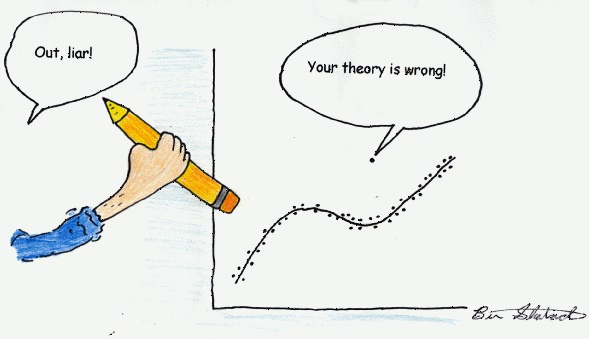
\includegraphics[width=0.8\textwidth]{lectOutliers/outlier_pic_1.jpg}
\footnote{Reprinted with permission 
\url{http://davidmlane.com/ben/cartoons.html}
}

Change your model to include the outlier!

\end{frame}
%***********************************************************
\begin{frame}{Why Look For Outliers?}

\begin{itemize}
	\item Classically, two reasons:
        		\begin{enumerate}
		\item  Classically, to remove them from data...
		\end{enumerate}
      		 \begin{itemize}
		\item ...because outliers can hurt learning process
        		\end{itemize}
        		\begin{enumerate}
		\setcounter{enumi}{1}
		\item  To find them for further examination...
		\end{enumerate}
        		\begin{itemize}
		\item ...because outliers might enhance \textcolor{red}{understanding} of data
        		\end{itemize}
        \item[?] What are some examples of applications where we want to find outliers?
\end{itemize}

\end{frame}
%***********************************************************
\begin{frame}{The Data Scientist's Goal}

\begin{itemize}
	\item Find the outliers!
        \begin{itemize}
	\item Computer security
	\item Fraud detection
	\item Medical crisis alerts
        \end{itemize}
\item[?] What if you find 1 MD prescribing lots of opioids. Is it fraud?
\end{itemize}



\end{frame}
%***********************************************************
\begin{frame}{The Data Scientist's Goal}

\begin{itemize}
	\item Find the outliers!
        \begin{itemize}
	\item Computer security
	\item Fraud detection
	\item Medical crisis alerts
        \end{itemize}
\item What if you find 1 MD prescribing lots of opioids. Is it fraud?
        \begin{itemize}
	\item Or is it a large practice and all the Rx's go under 1 name?
        \end{itemize}

\end{itemize}



\end{frame}
%***********************************************************
\begin{frame}{Supervised vs. Unsupervised Learning}

\begin{itemize}
	\item Supervised learning -- labels are provided
	\item Unsupervised learning -- no labels  provided
\end{itemize}

\end{frame}
%***********************************************************
\begin{frame}{Outlier Detection is an Unsupervised Task}

\begin{itemize}
	\item[?] Why?
\end{itemize}

\end{frame}
%***********************************************************
\begin{frame}{Outlier Detection is an Unsupervised Task}

\begin{itemize}
	\item Why?
        \begin{itemize}
        \item We don't always know what the outliers look like
        \item By definition, we don't expect them
        \item They are rare
        \end{itemize}
        \item Supervised learning requires labels
\end{itemize}



\end{frame}
%***********************************************************
\begin{frame}{How Do We Define Outliers?}

\begin{itemize}
\item Two standard definitions:
        \begin{itemize}
	\item (1) Distance-based
	\item (2) Model-based
        \end{itemize}
\end{itemize}

\end{frame}
%***********************************************************
\begin{frame}{Distance Based Outlier Detection}

\begin{itemize}
\item Classical approach
\item Most frequently used
\item Feasible - if we have a high dimensional space, outliers are very far from the other points
\end{itemize}

\end{frame}
%***********************************************************
\begin{frame}{Model Based Outlier Detection}

\begin{itemize}
\item Requires a proper statistical model
\item If a data point has a very low probability of occurring, flag that
        \begin{itemize}
	\item Coin flips:
	\item 10 flips: 9 heads 
	\item[?] Is our coin biased?
        \end{itemize}
\end{itemize}
\end{frame}
%***********************************************************
\begin{frame}{Model Based Outlier Detection}

\begin{itemize}
\item Requires a proper statistical model
\item If a data point has a very low probability of occurring, flag that
        \begin{itemize}
	\item Coin flips:
	\item 10 flips: 9 heads 
	\vspace{1em}
	\item  $10 * \frac{1}{2}^9 * (1 -\frac{1}{2}) = 10 * \frac{1}{2}^{10} = 0.00977 $
	\item 10 * P(heads) * P(Tails)
	\item Your coin is likely biased
        \end{itemize}
\end{itemize}
\end{frame}
%***********************************************************
\begin{frame}{kNN}

\begin{itemize}
\item $k$ Nearest Neighbors
\item Very popular machine learning algorithm
\item Relatively simple
        \begin{itemize}
	\item Look at a data point
	\item Consider the $k$ closest points to it
	\item Make a decision based on that information
\end{itemize}
\end{itemize}
\end{frame}
%***********************************************************
\begin{frame}{Distance-Based Outliers}

\begin{itemize}
	\item Definition: A point is an outlier if it is far from all other points
	\vspace{1 em}
	\item Outlier search often defined in terms of $k$NN:
	\begin{itemize}
	\item Let $d(x_i)$ be the distance to point $x_i$'s $k$thNN in the data set
	\item Then, given data set $\langle x_1, x_2, ..., \rangle$, 
		we want to compute the set $O$ of outliers such that...
	\item $|O| = m$ the number of points in the set is $m$
	\item and $\forall (x_o \in O, x_i \in \textbf{X} - \textbf{O}), d(x_o) \ge d(x_i)$
	\vspace{1 em}
	\item That is, for every point $x_o$ in our outlier set
	\item and \textbf{every} point $x_i$ \textbf{NOT} in our outlier set
	\item the outlier distance is further than the non-outlier distance 
	\end{itemize}
\end{itemize}

\end{frame}
%***********************************************************
\begin{frame}{How to Find Distance-Based Outliers, Conceptually (2NN)?}

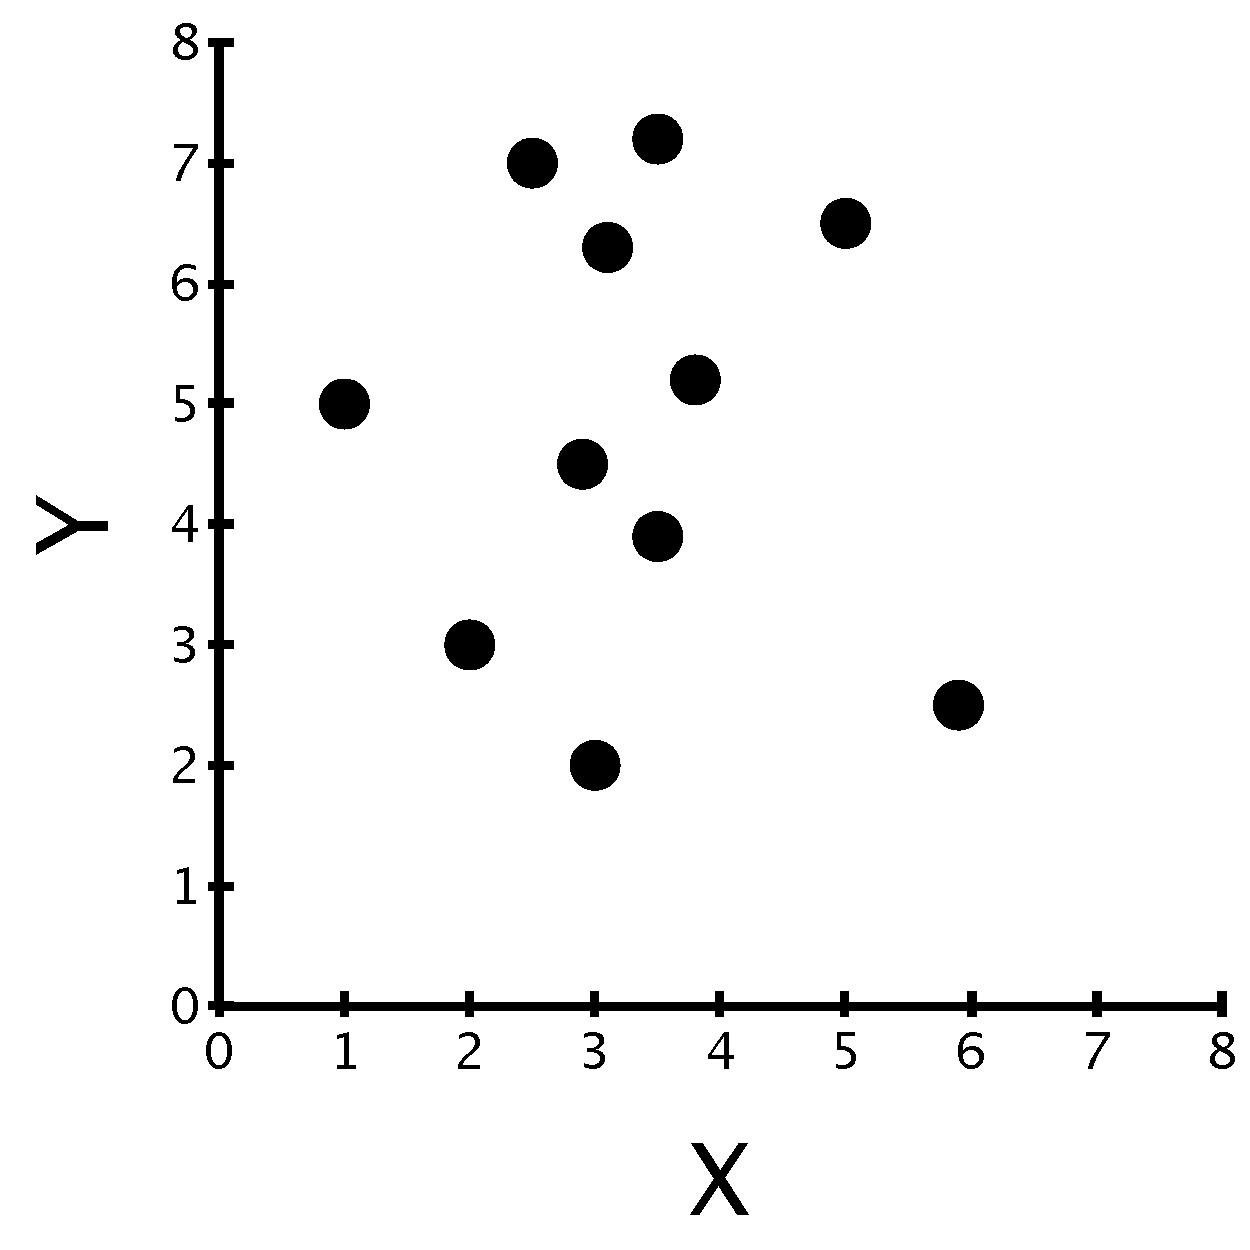
\includegraphics[width=0.5\textwidth]{lectOutliers/outliersPts.pdf}


\end{frame}
%***********************************************************
\begin{frame}{Pick a Point (2NN)}

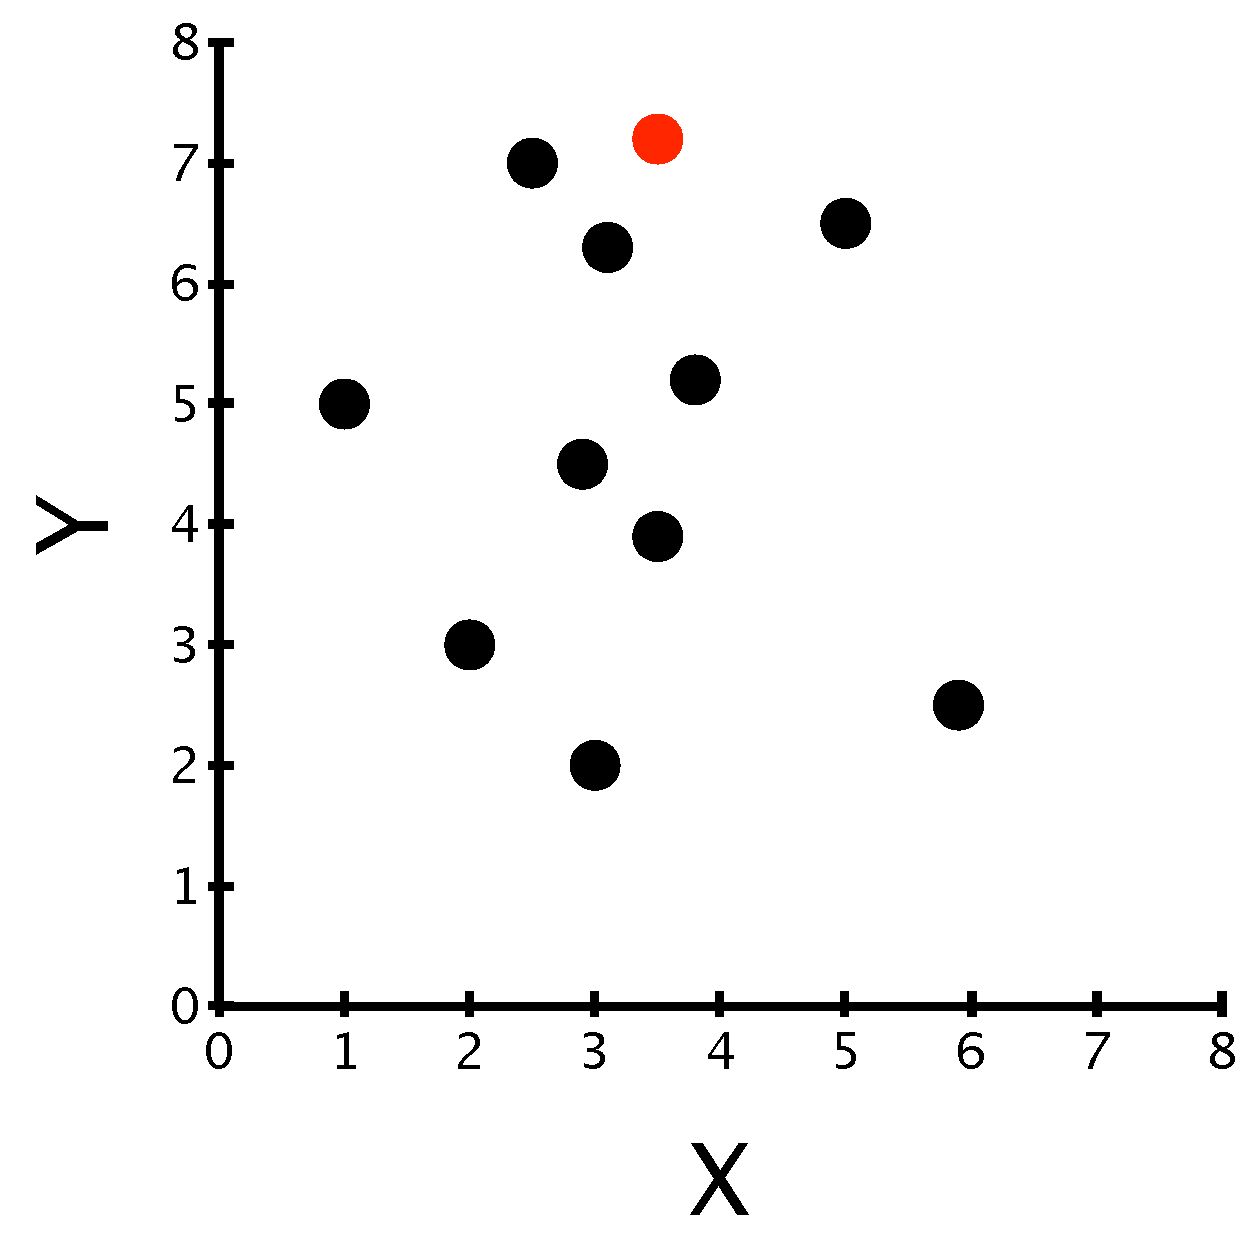
\includegraphics[width=0.5\textwidth]{lectOutliers/outliersPtsA.pdf}

\end{frame}
%***********************************************************
\begin{frame}{Compute Distance to All Other Points (2NN)}

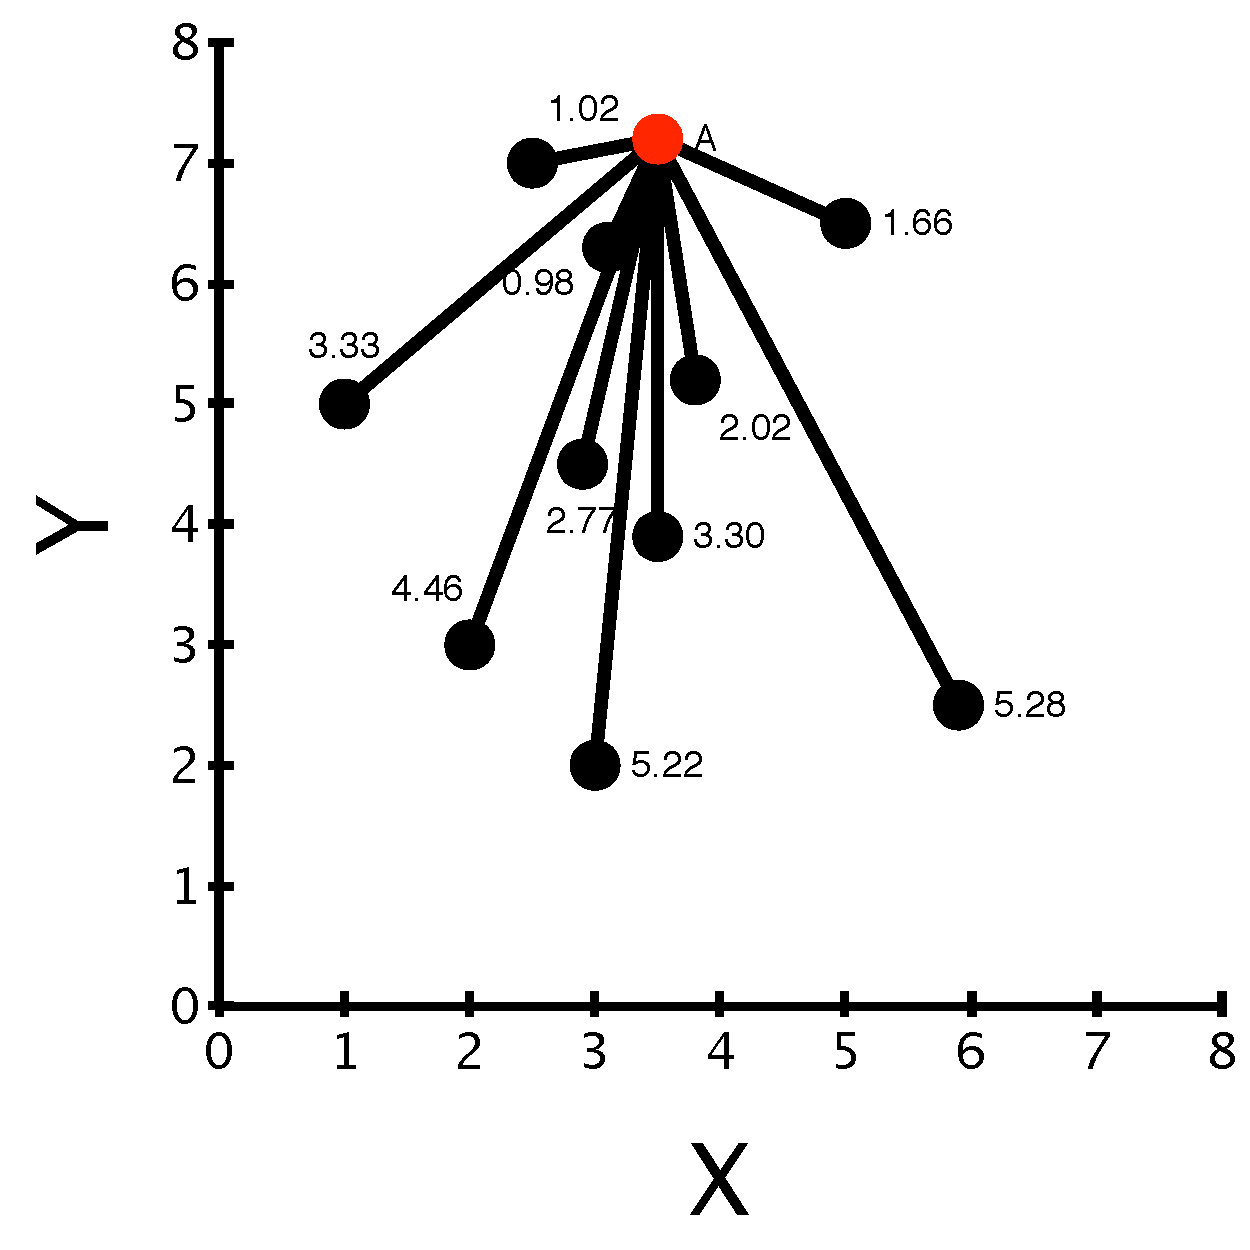
\includegraphics[width=0.5\textwidth]{lectOutliers/outliersPtsAAll.pdf}

\end{frame}
%***********************************************************
\begin{frame}{Find the Distance to the 2nd NN (2NN)}

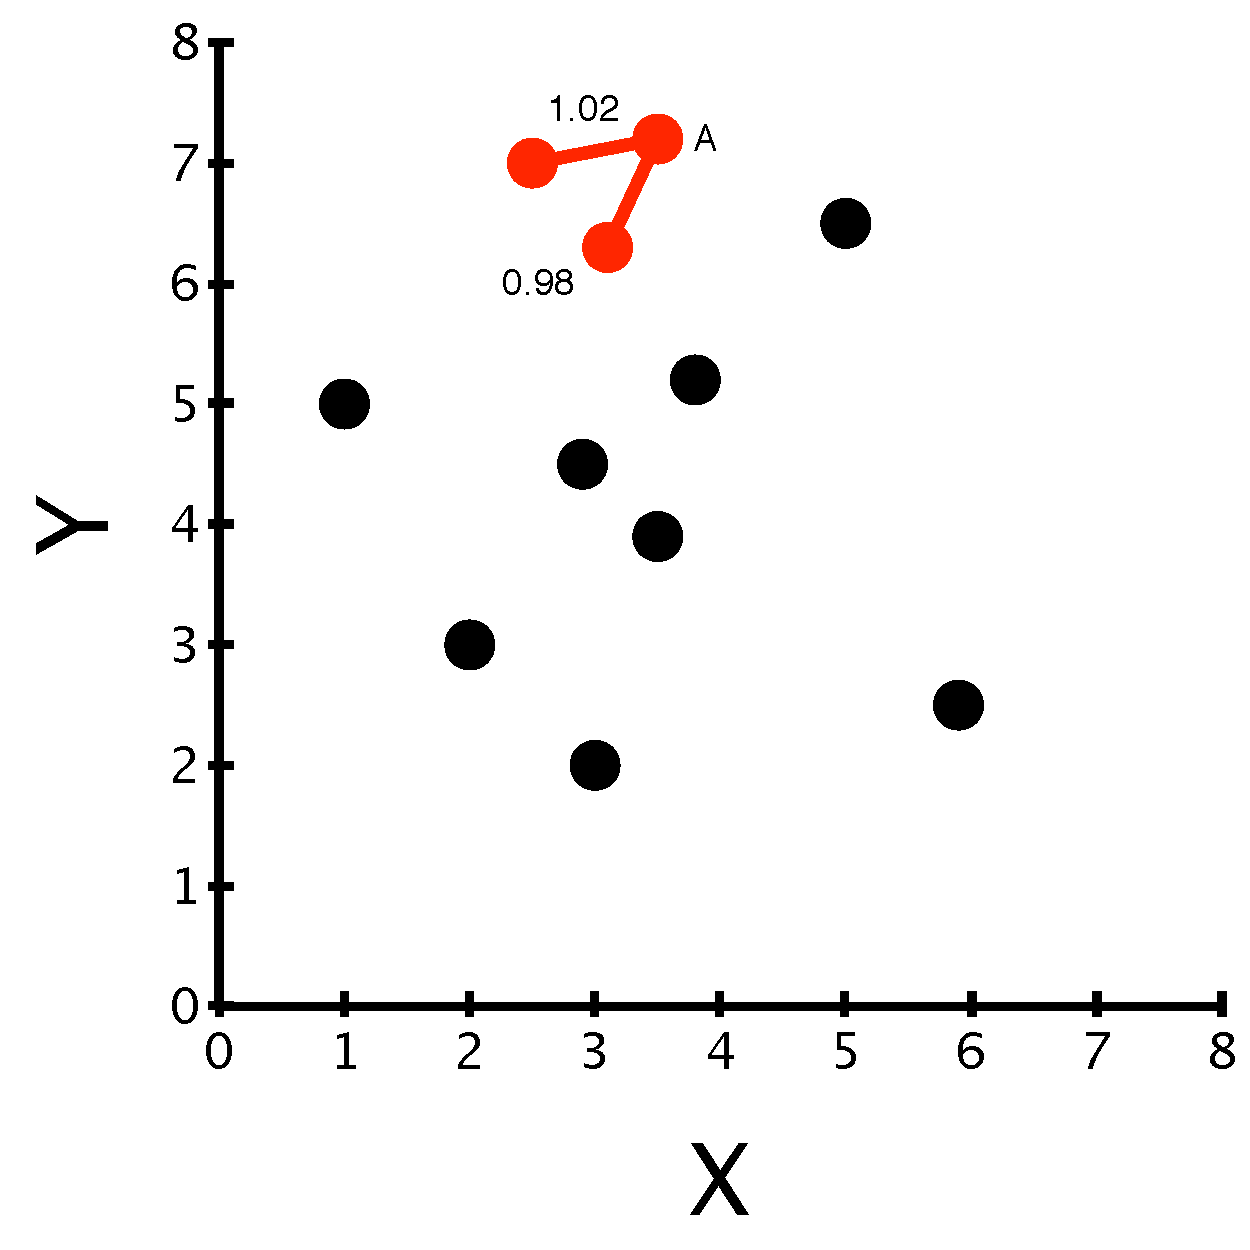
\includegraphics[width=0.5\textwidth]{lectOutliers/outliersPtsA2NN.pdf}

\end{frame}
%***********************************************************
\begin{frame}{Repeat for All Points}

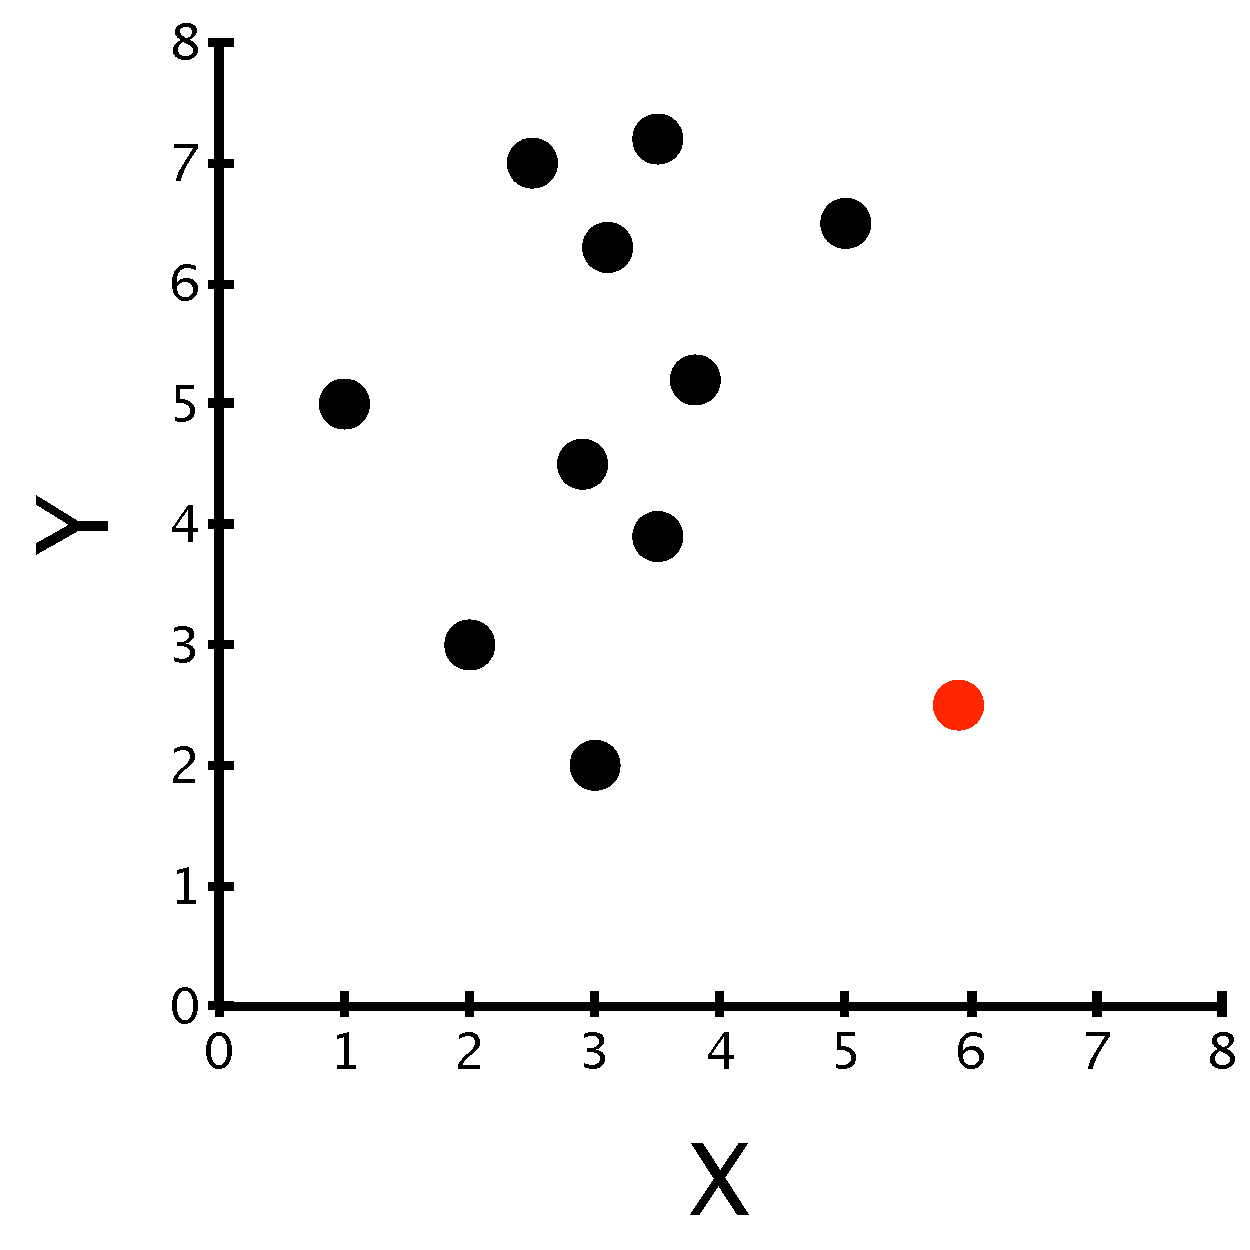
\includegraphics[width=0.5\textwidth]{lectOutliers/outliersPtsO1.pdf}
\end{frame}
%***********************************************************
\begin{frame}{Finding the 2nd NN Distance}

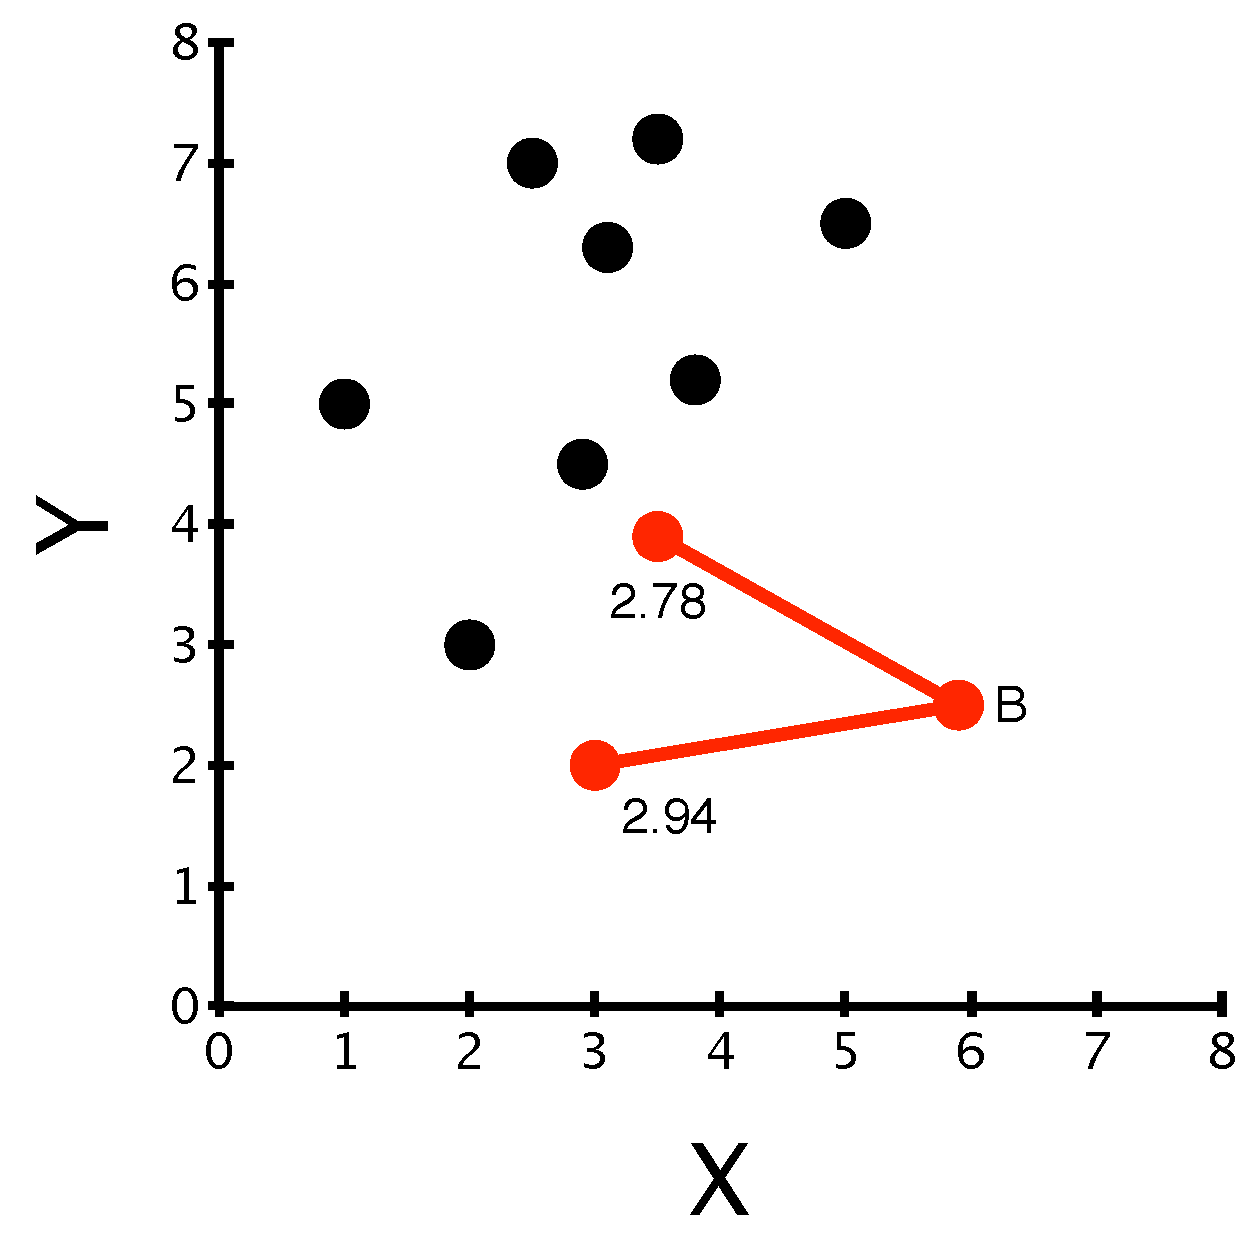
\includegraphics[width=0.5\textwidth]{lectOutliers/outliersPtsO2.pdf}
\end{frame}
%***********************************************************
\begin{frame}{Select the Top m "Outlierly" Points}
%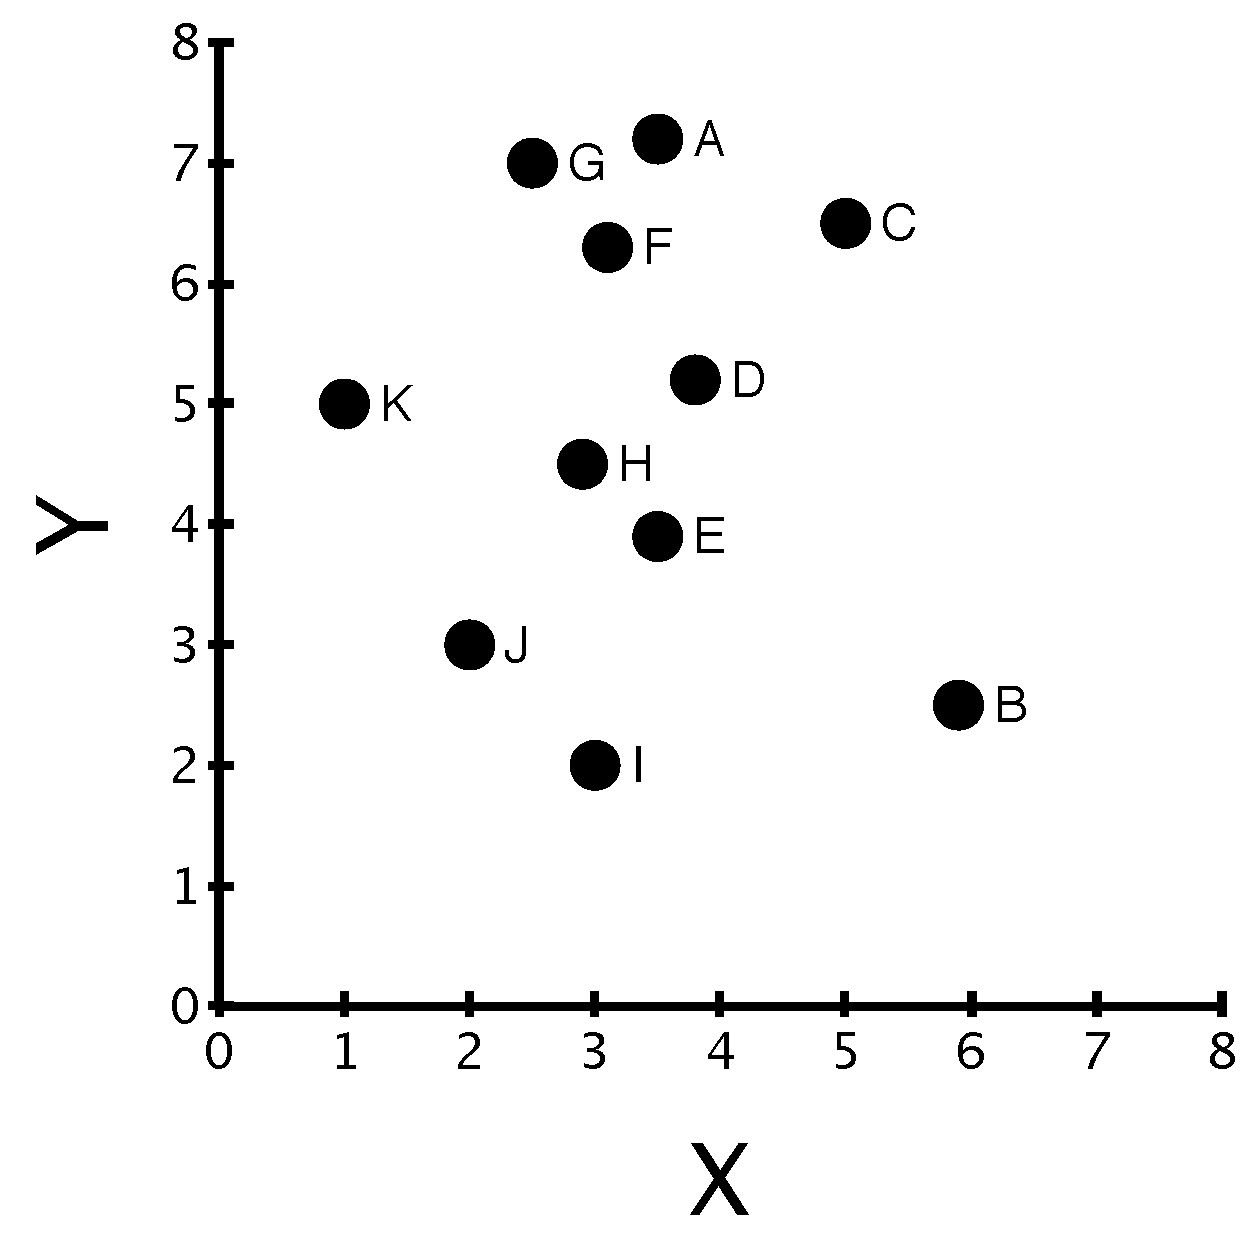
\includegraphics[width=0.5\textwidth]{outliersPtsLabeled.pdf}

\begin{figure}[ht]
\begin{minipage}[b]{0.5\linewidth}
\centering
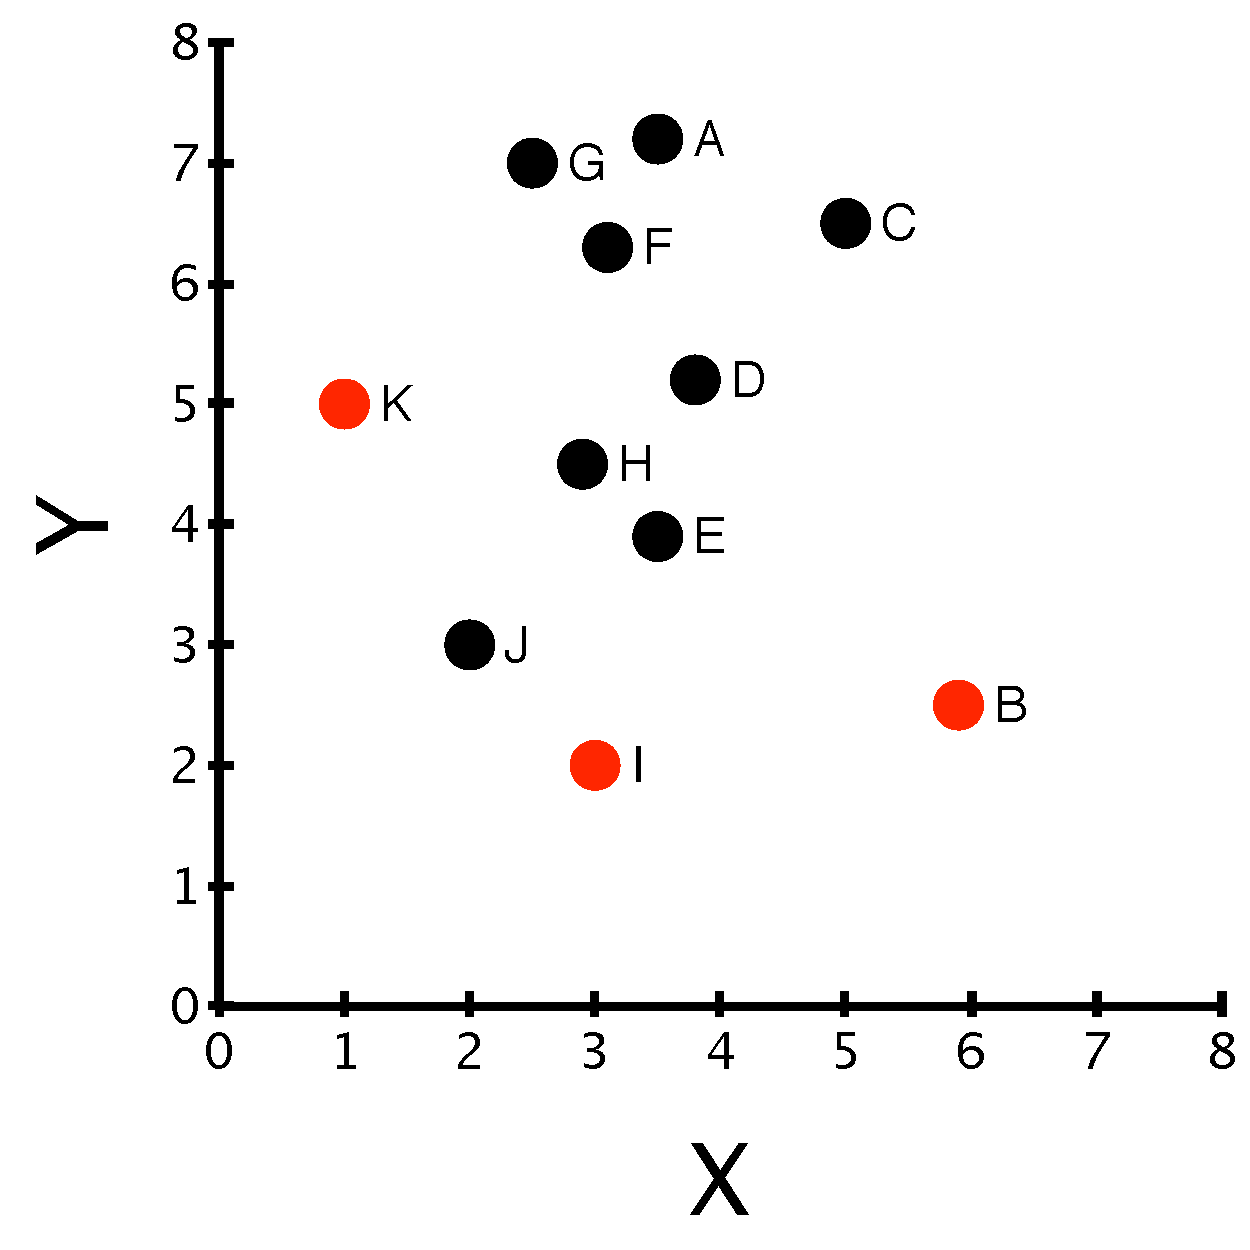
\includegraphics[width=\textwidth]{lectOutliers/outliersPtsLabeled3Most.pdf}
\end{minipage}
\hspace{0.5cm}
\begin{minipage}[b]{0.4\linewidth}
\centering
\small{
\begin {table}[!htbp]
\begin{center}
\begin{tabular}{|r|r|}
\hline
Point & 2NN distance \\ \hline
A & 1.02 \\ \hline
\textcolor{red}{B} & \textcolor{red}{2.94}  \\ \hline
C & 1.77 \\ \hline
D & 1.30 \\ \hline
E & 1.33  \\ \hline
F & 0.98 \\ \hline
G & 1.02 \\ \hline
H & 1.14 \\ \hline
\textcolor{red}{I} & \textcolor{red}{1.96} \\ \hline
J & 1.75 \\ \hline
\textcolor{red}{K} & \textcolor{red}{2.24} \\ \hline
\end{tabular}
\end{center}
\end{table}
}

\end{minipage}
\end{figure}

\end{frame}
%***********************************************************
\begin{frame}[fragile]{How To Find Distance-Based Outliers?}


\begin{itemize}
\item Simple algorithm: 
        \begin{itemize}
	\item O is the set of current Outliers
	\item Q is the closest distances to the current point
        \end{itemize}
\end{itemize}
\vspace{-1em}
\begin{SQL}
init min-priority queue $O$
for $x_1 \in X$:
  init max-priority queue $Q$
  for $x_2 \neq x_1 \in X$:
    insert $dist(x_1, x_2)$ into $Q$
    if $|Q| > k$
      remove max from $Q$
  insert $x_1$ into $O$ with key max$(Q)$
  if $|O| > m$
    remove point with min key from $O$

return $O$ 
\end{SQL}

\begin{itemize}
\item $m$ is the number of outliers we are looking for
\item $k$ is the nearest neighbor we consider
\item Let's walk through an example in detail
\end{itemize}

\end{frame}
%***********************************************************
\begin{frame}[fragile]{How To Find Distance-Based Outliers?}
\begin{itemize}
\item So, this works!
\item[?] Are there any problems here?
\end{itemize}

\end{frame}
%***********************************************************
\begin{frame}{How To Find Distance-Based Outliers?}

\begin{itemize}
\item What are the problems here?
	\begin{itemize}
	\item $m$ \& $k$ are magic/arbitrary numbers
	\item Nested loop thru entire database O(N$^2$)
	\item Too slow for big data
	\item How to address (the computational problem)?
	\end{itemize}
\end{itemize}
% a billion squared is just too many
% have to compare every point against each other
% can be a little smarter (1/2 as many comparisons if we loop over higher indexes)

% we'll come back to m & k later
\end{frame}
%***********************************************************
\begin{frame}[fragile]{How To Find Distance-Based Outliers?}

\begin{itemize}
\item Better algorithm: 
       \begin{itemize}
	\item O is the set of current Outliers
	\item Q is the closest distances to the current point
        \end{itemize}
\end{itemize}
\begin{columns}
\begin{column}{0.5\textwidth}
\begin{SQL}
init min-priority queue $O$
for $x_1 \in X$:
  init max-priority queue $Q$
  for $x_2 \neq x_1 \in X$:
    insert $dist(x_1, x_2)$ into $Q$
    if $|Q| > k$
      remove max from $Q$
    if $|Q| == k$ and $|O| == m$ and max$(Q)$ < min$(O)$ 
      discard $x_1$; not an outlier
  insert $x_1$ into $O$ with key max$(Q)$
  if $|O| > m$
    remove point with min key from $O$

return $O$ 
\end{SQL}
\end{column}
\begin{column}{0.4\textwidth}
\begin{itemize}
\item $Q$ \& $O$ must be full
\item If I find a neighbor who is closer than the current outlier distance, I \textbf{can't} be a top outlier
\item So move to the next candidate point
\end{itemize}
\end{column}
\end{columns}

% if I find a neighbor that is closer than the current outlier distance, I can't be a top outlier, so move to next candidate point
% the distance to my nearest neighbors can only go down from MAX(Q), so it's ok to prune

% even tho still O(N^2)
% can have > 100x speed up
\end{frame}
%***********************************************************
\begin{frame}{How To Find Distance-Based Outliers?}

\begin{figure}[ht]
\begin{minipage}[c]{0.4\linewidth}
\begin{itemize}
\item Why does this help?
	\begin{itemize}
	\item \texttt{max}$(Q)$ is an upper bound on distance to $k$th NN
	\item So distance to $k$th NN can't ever be greater
	\item If this is not good enough to get point into top $m$ in $O$
	\item Then can discard it early
	\end{itemize}
\end{itemize}
%\centering
\end{minipage}
\hspace{0.5cm}
\begin{minipage}[c]{0.5\linewidth}
%\centering
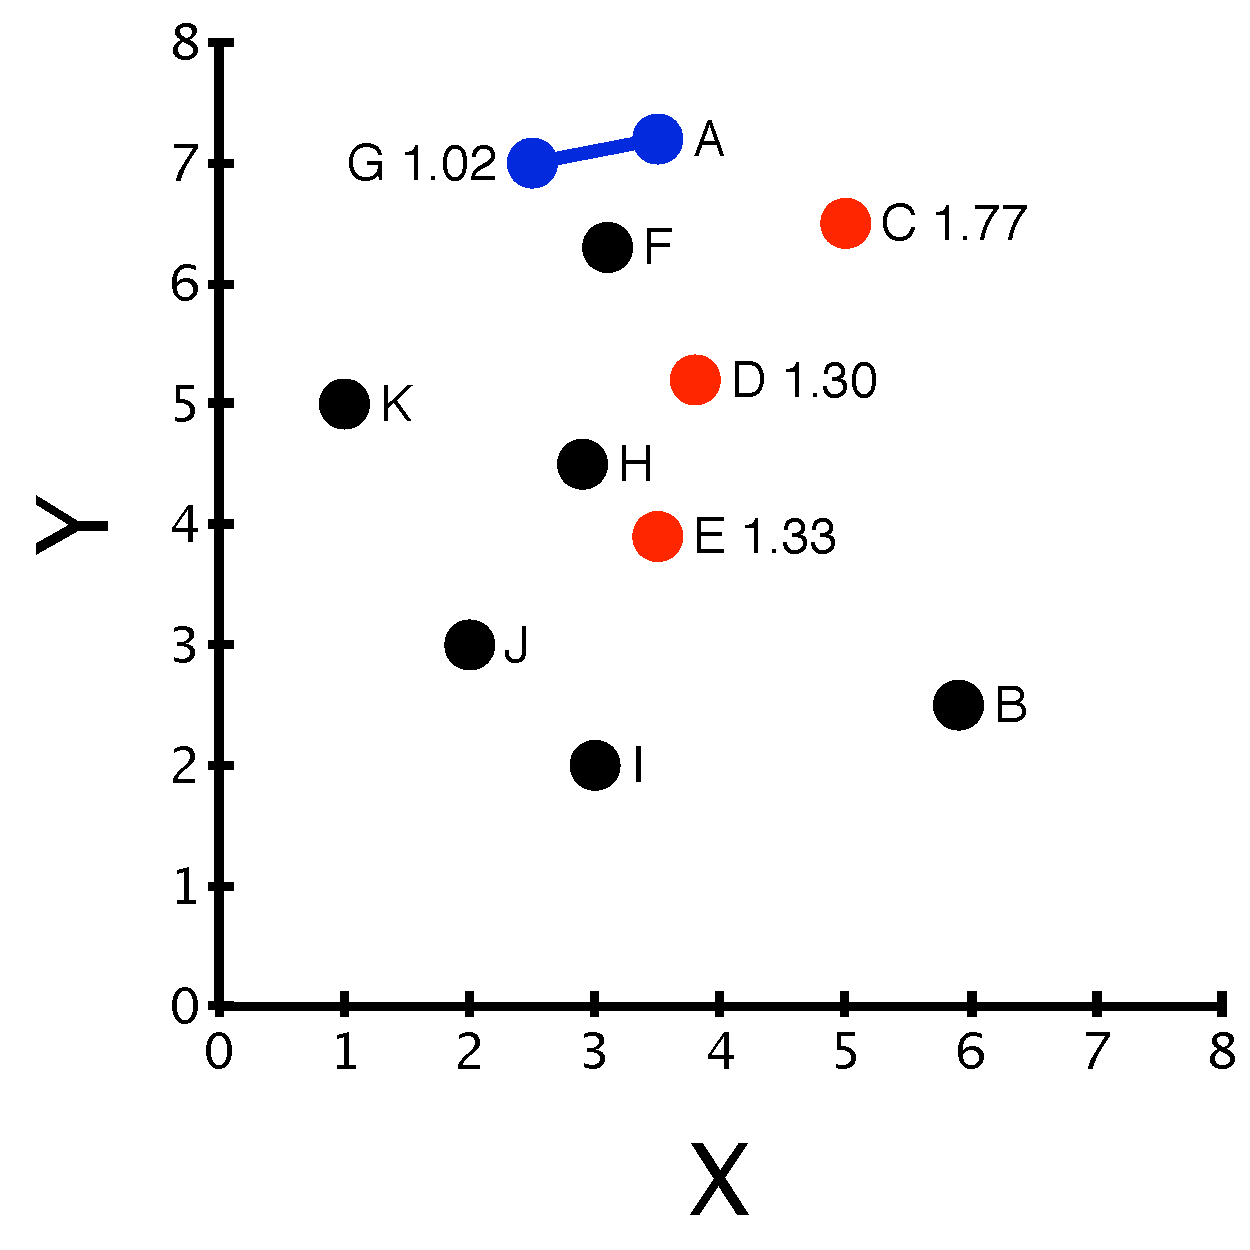
\includegraphics[width=\textwidth]{lectOutliers/outliersPtsLabeledBetterAlg.pdf}
\end{minipage}
\end{figure}
\end{frame}
%***********************************************************
\begin{frame}{How To Find Distance-Based Outliers?}

\begin{figure}[ht]
\begin{minipage}[c]{0.4\linewidth}
\begin{itemize}
\item Example:  O: \{(1.33, E), (1.77, C) (1.30, D) \}
	\begin{itemize}
	\item Process F
	\item Find 2NN $distance(F,A) = 0.98$
	\item $0.98 < 1.30$ so discard F
	\end{itemize}
\item Can get a 100x speed up
\item But, it's still $O(N^2)$
\end{itemize}
%\centering
\end{minipage}
\hspace{0.5cm}
\begin{minipage}[c]{0.5\linewidth}
%\centering
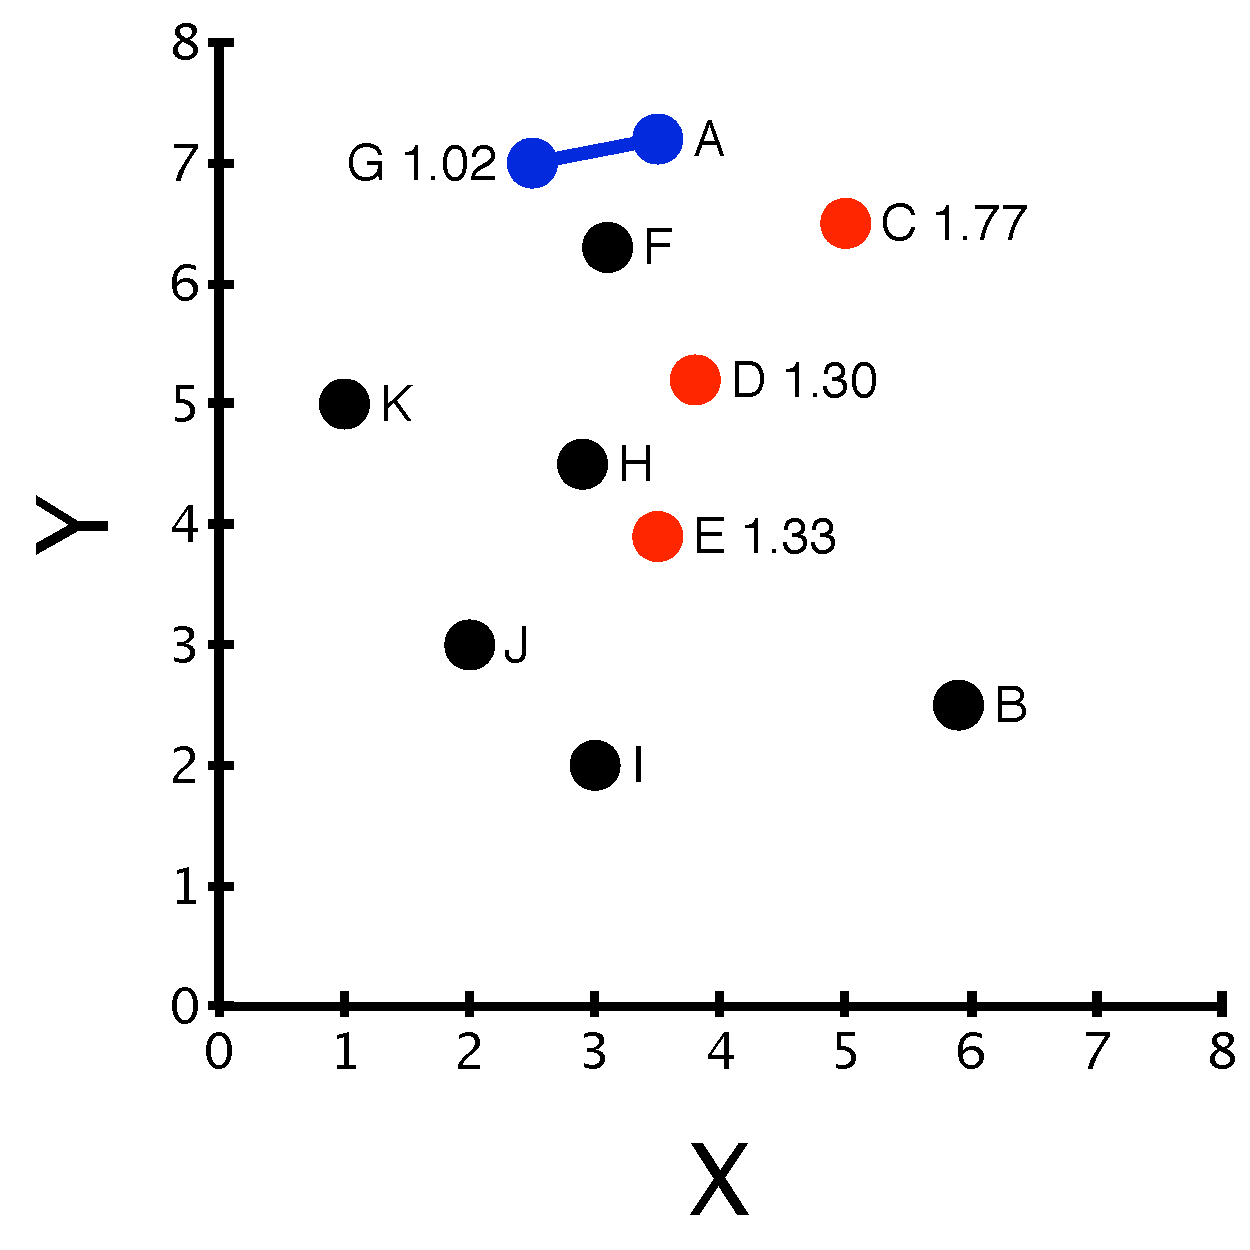
\includegraphics[width=\textwidth]{lectOutliers/outliersPtsLabeledBetterAlg.pdf}
\end{minipage}
\end{figure}


% Ex: O: {(1.33, E), (1.77, C) (1.30, D) }
% processing F, and find that 2NN dist(F, A) = 0.98
% Can stop processing F



\end{frame}

%***********************************************************
\begin{frame}{How To Find Distance-Based Outliers?}

\begin{itemize}
\item Even better:
	\begin{itemize}
	\item Store $X$ in randomized order
	\item That way, won't get unlucky and find all far points first
%	\item (Imagine 1-d data, sorted on key)
	\end{itemize}
\end{itemize}

% Create example!

% Say the LAST 3 points we check are the top 3 outliers. Then, we have to fully check all the other pairwise distances  to be sure nothing else is better


\end{frame}
%***********************************************************
%\begin{frame}{What About the Distance}
%
%\begin{itemize}
%\item I'll steal a slide from an old lecture...
%\item How to compute $dist(x, y)$?
%        \begin{itemize}
%        \item Classical method: if $x$, $y$ vectors, use $l_p$ norm of $x - y$
%        \item Drawbacks?
%        \end{itemize}
%\item Mahalanobis distance is more robust
%        \begin{itemize}
%        \item Let $\mu$ be the mean vector of the data set
%        \item Let $S$ be the observed covariance matrix of data set
%        \item That is, let $X$ be the matrix where the $i$th row is $x_i - \mu$
%        \item Then $S = \frac{1}{n - 1} X^T X$
%        \item Mahalanobis computed as:
%                $$ d(x, y) = \left((x - y)^T S^{-1} (x - y)\right)^{\frac{1}{2}}$$
%        \end{itemize}
%\end{itemize}
%\end{frame}
%***********************************************************
\begin{frame}{How to Choose m and k?}

\begin{itemize}
\item What goes into m?
	\begin{itemize}
	\item Size of the data set
	\item Ability of humans to process / deal with the identified outliers
	\item Start small and make m bigger. Stop when nothing ``interesting'' is added
	\item Very application specific
	\end{itemize}
\item What goes into k?
	\begin{itemize}
	\item Size of the data set
	\item How far apart are your data? k ``smooths" the data. % get photo http://scott.fortmann-roe.com/docs/BiasVariance.html
	\item Try $\sqrt{N}$
	\item Determine empirically using your validation set
	\end{itemize}
\end{itemize}

\end{frame}
%***********************************************************
\begin{frame}{Model-Based Outliers}
\begin{itemize}
\item Basic idea:
	\begin{itemize}
	\item Learn a model for what is ``typical''
%	\item Might be probabilisitic
%	\item Might be least-squares
	\item Then outlier is data point with low score according to the model
	\end{itemize}
\end{itemize}

\end{frame}
%***********************************************************
\begin{frame}{Example of Model-Based Detection}

\begin{itemize}
%\item Learn parameters of a GMM by choosing $\pi, \{\mu\}, \{\sigma^2\}$ to max
%$$P(x_1, x_2, ..., x_n) = \prod_i \left( \sum_j \pi_j \textrm{Normal} (x_i | \mu_j, \sigma^2_j) \right)$$
%\item Then choose $m$ points with smallest $\sum_j \pi_j \textrm{Normal} (x_i | \mu_j, \sigma^2_j)$
\item Learn parameters of a Normal distribution by choosing $\mu, \sigma^2$ to maximize
$$P(x_1, x_2, ..., x_n) = \prod_i \left( \textrm{Normal} (x_i | \mu, \sigma^2) \right)$$
\item Then choose $m$ points with highest $\textrm{Normal} (x_i | \mu, \sigma^2) $ PDF
\item Whichever points are not described well by the model are considered outliers
\end{itemize}

\begin{columns}
\begin{column}{0.4\textwidth}
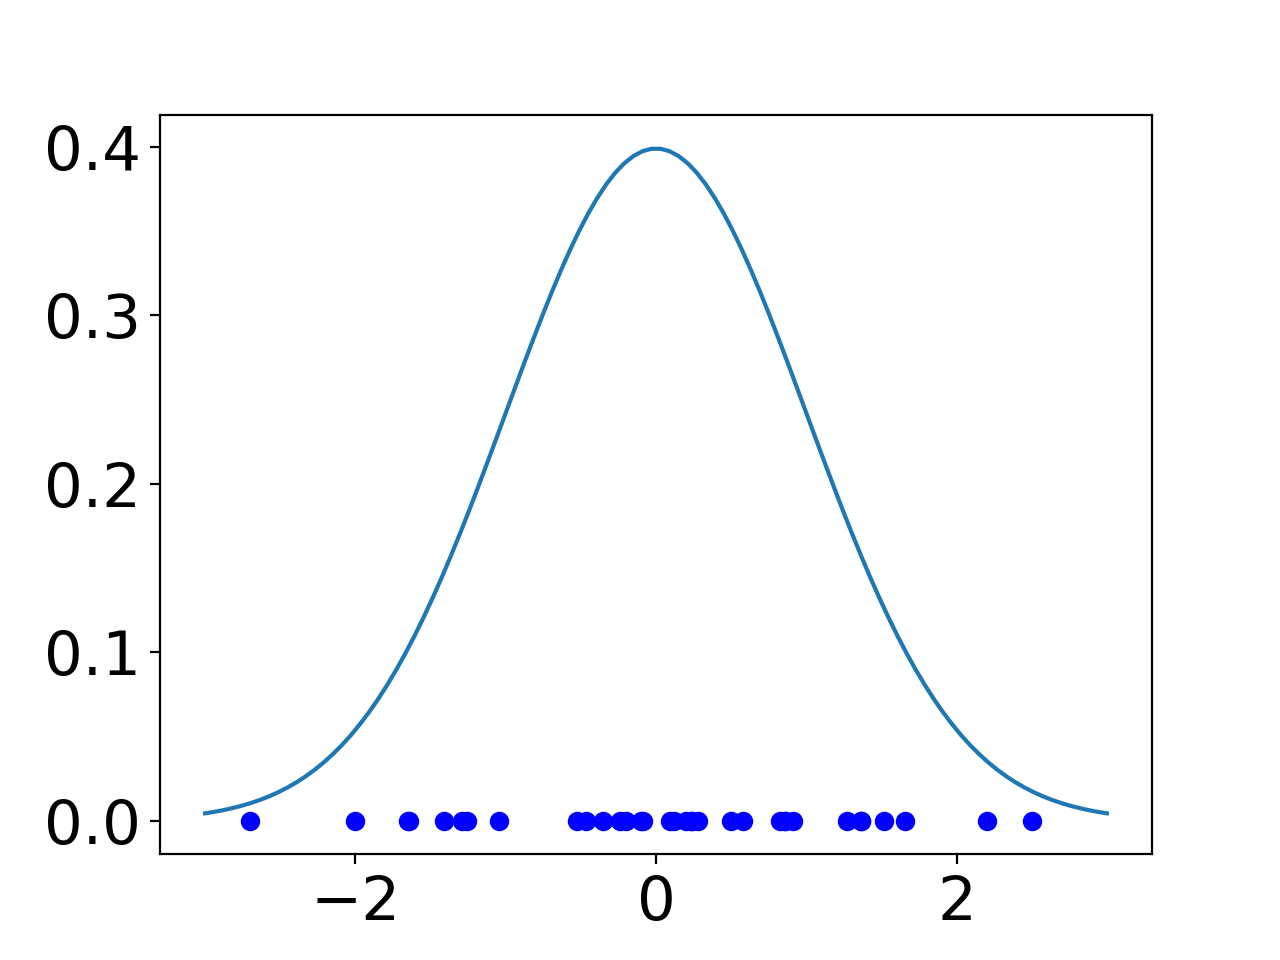
\includegraphics[width=\textwidth]{lectOutliers/normalModel.png}
\end{column}
\begin{column}{0.6\textwidth}
\begin{itemize}
\item Most likely data occurs in the middle, points in the tails are less likely
\end{itemize}
\end{column}
\end{columns}


\end{frame}
%***********************************************************
%\begin{frame}{Another Example of Model-Based Outlier Detection}
%
%\begin{itemize}
%\item Learn an SVM that distinguishes between the origin and all other data points
%\begin{itemize}
%	\item Called a ``one-class'' SVM
%	\item Then points are scored as outliers if they cross the decision boundary
%	\item Or are close to the decision boundary
%	\item[?] Any issues with this approach?
%\end{itemize}
%\end{itemize}
%\begin{columns}
%\begin{column}{0.35\textwidth}
%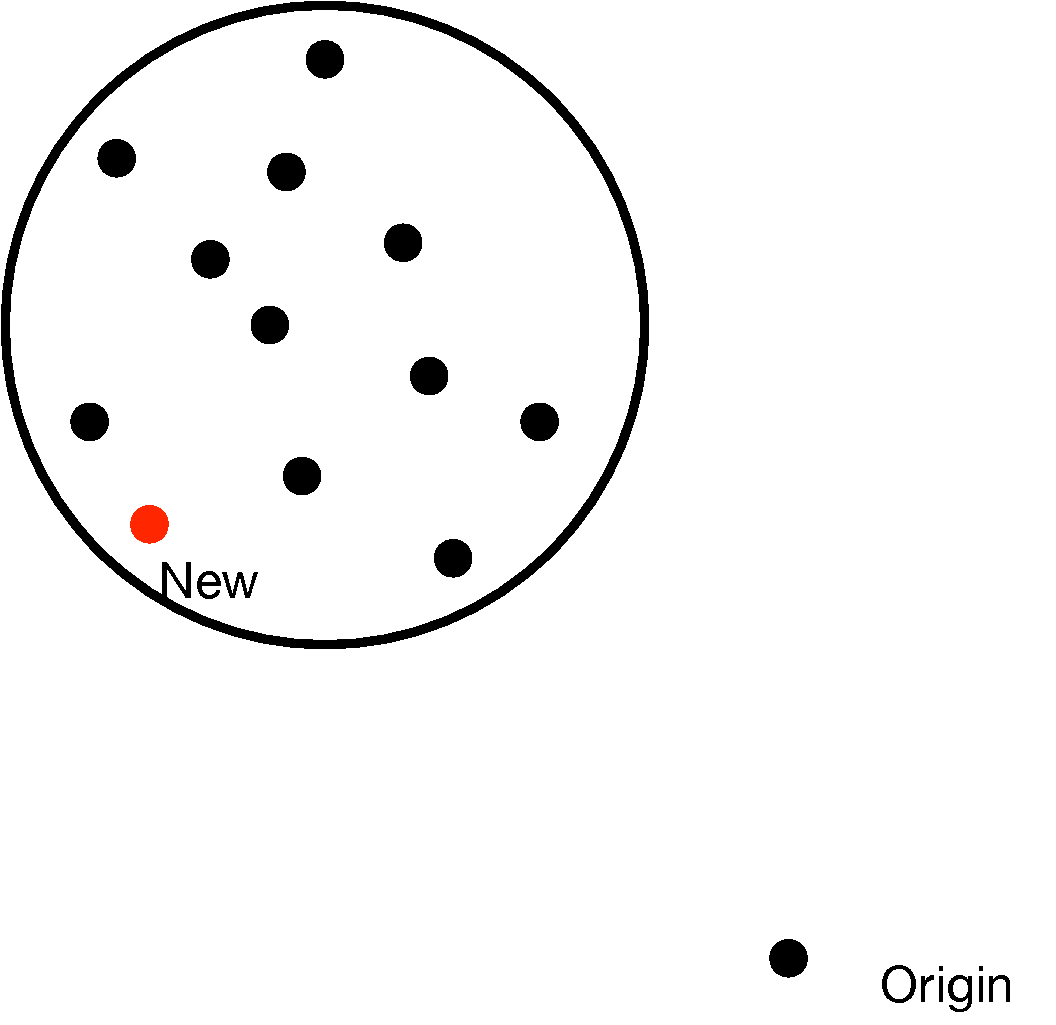
\includegraphics[width=\textwidth]{lectOutliers/oneClassSVM1.pdf}
%\end{column}
%\begin{column}{0.35\textwidth}
%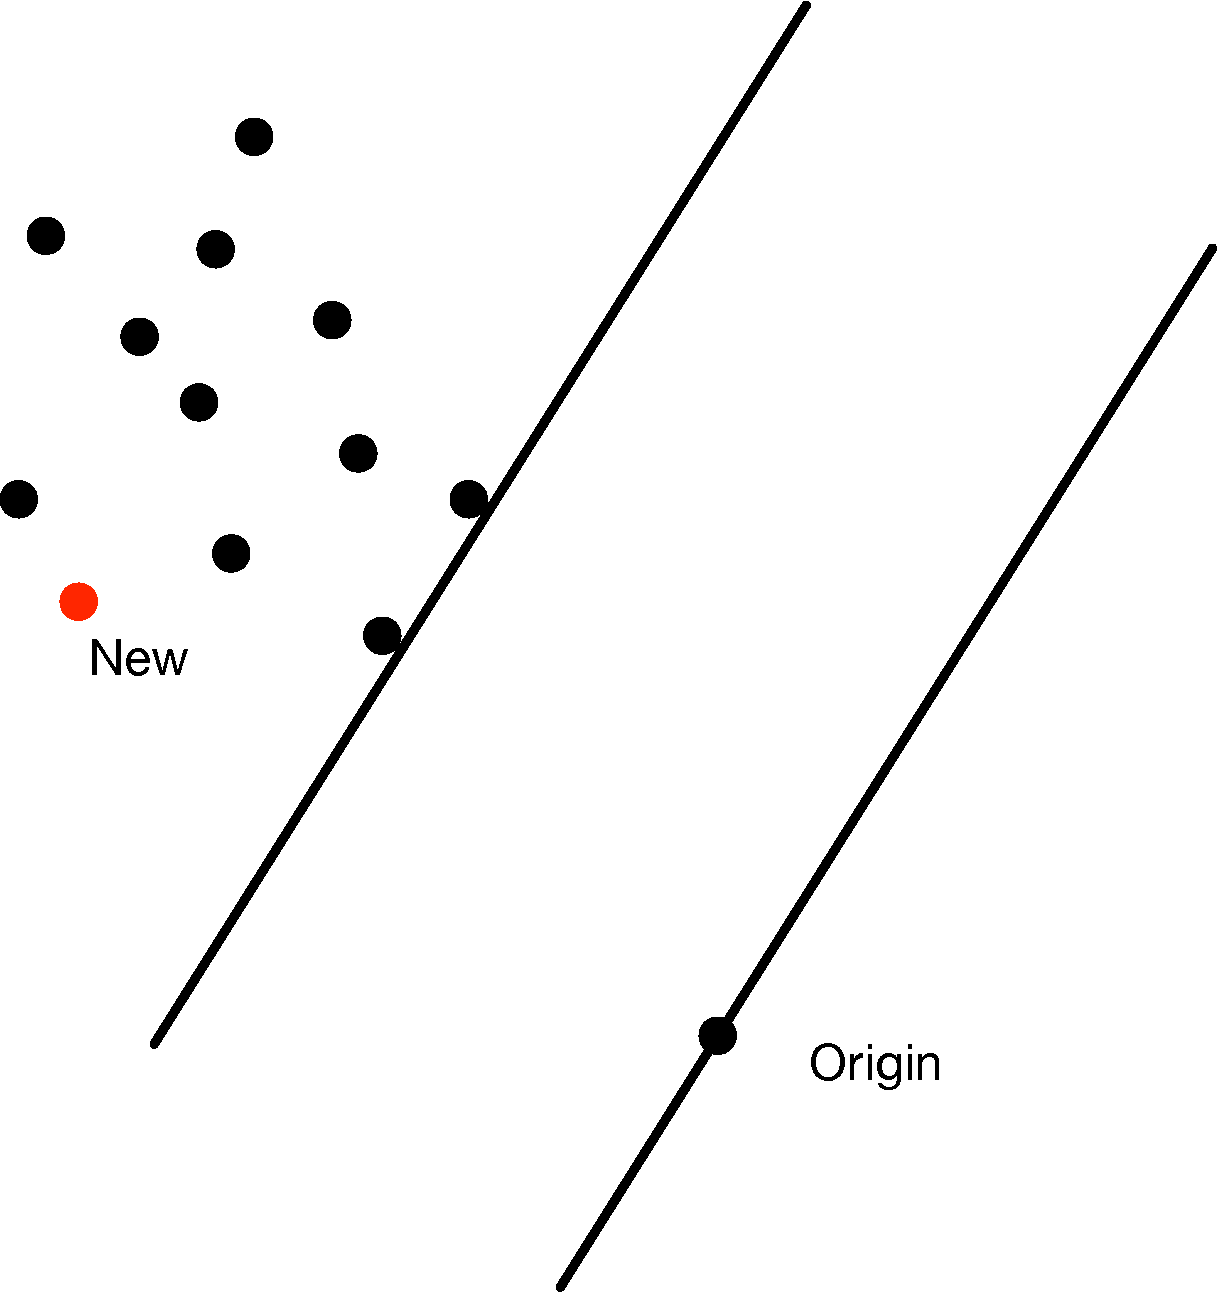
\includegraphics[width=\textwidth]{lectOutliers/oneClassSVM2.pdf}
%\end{column}
%\end{columns}
%
%% plane wraps around the class of points
%% puts all the data in 1 class
%% Pick a non-data point (usually the origin)
%% Test whether or not a new point is in or out of the set
%
%\end{frame}
%%***********************************************************
%\begin{frame}{Issue with One Class SVM?}
%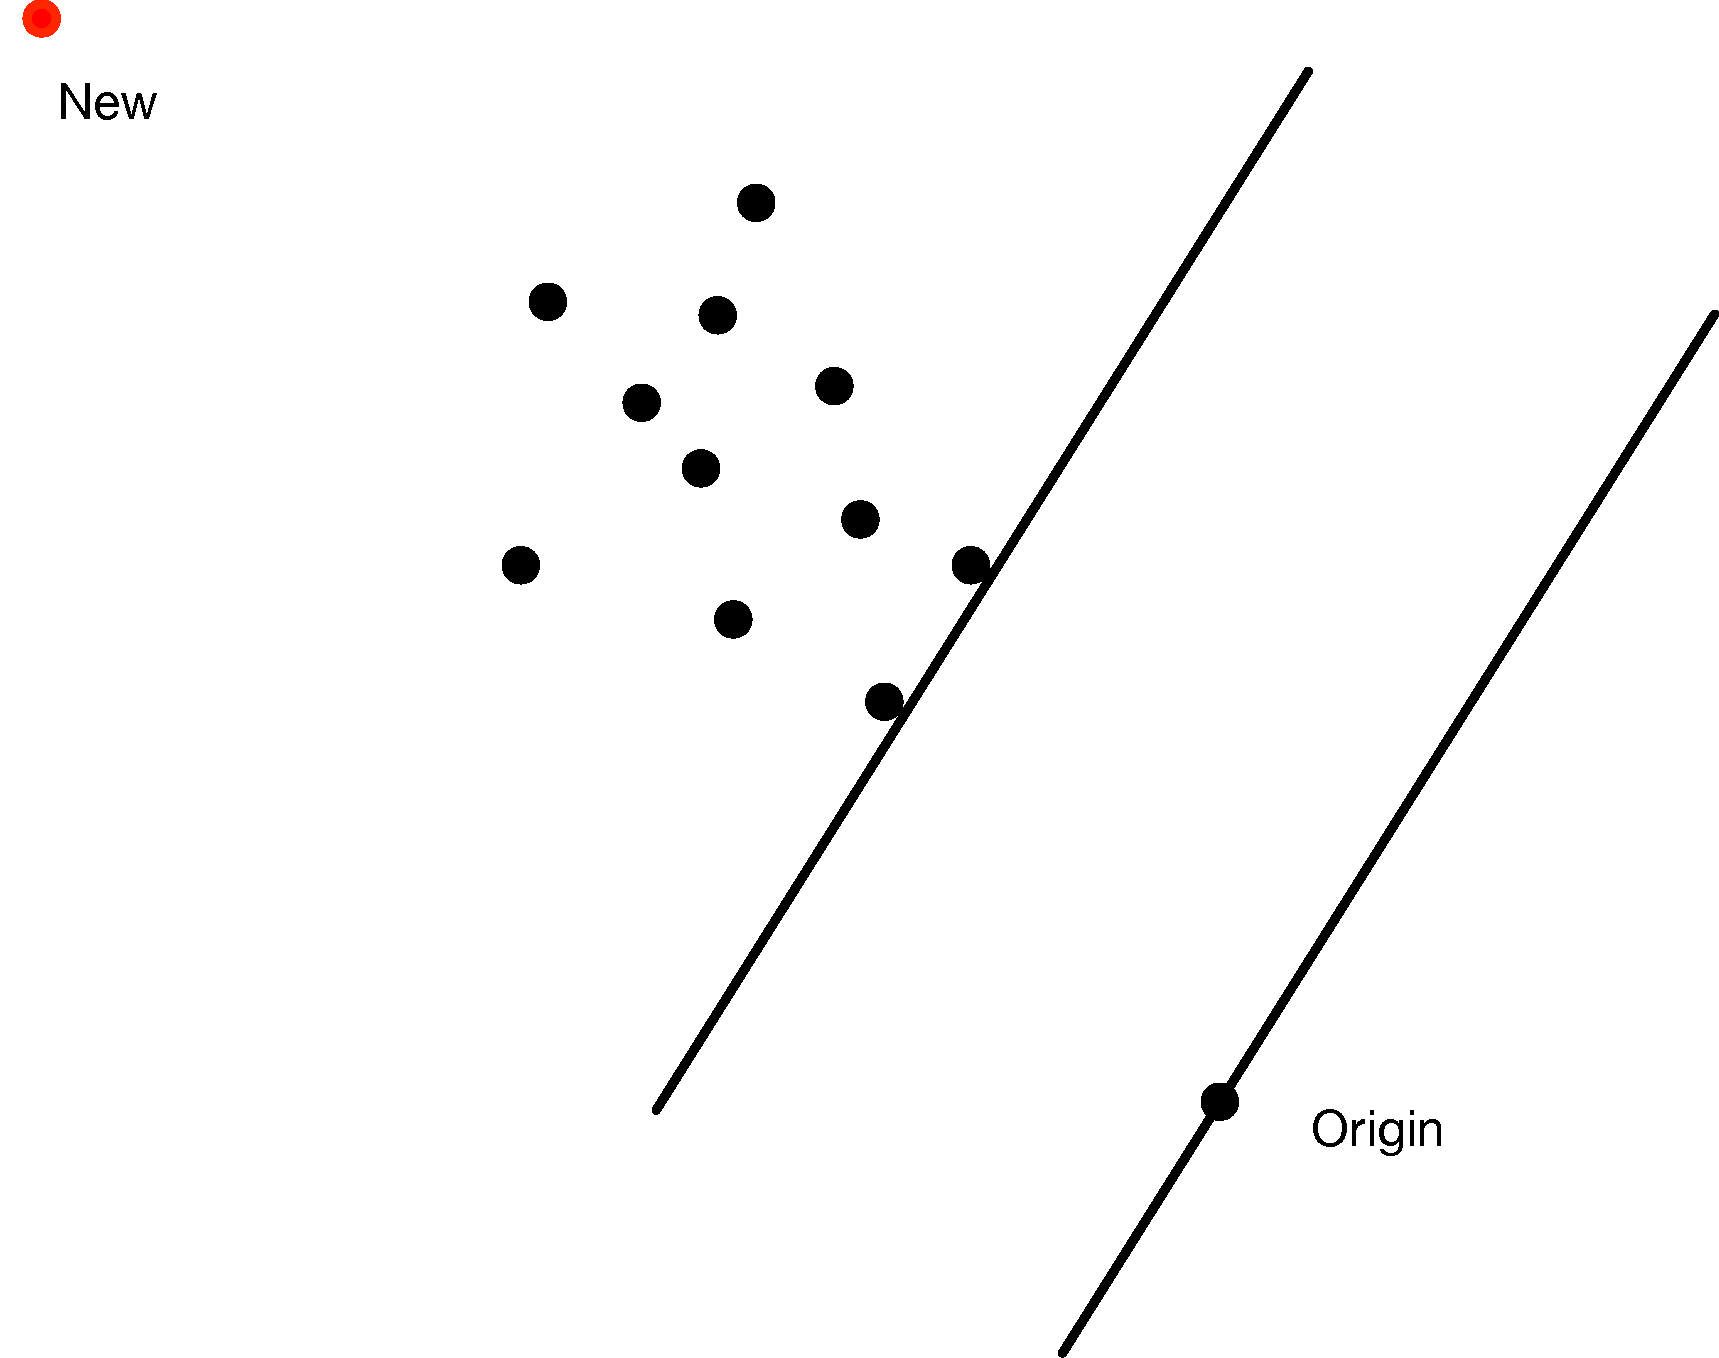
\includegraphics[width=.75\textwidth]{lectOutliers/oneClassSVMmissedOutlier.pdf}
%\end{frame}
%
%***********************************************************
\begin{frame}{Use Case Real-time Detection}

\begin{itemize}
\item Write software to sound an alarm 
% could be intruder alert, could be medical emergency
\item Use existing dataset to identify a \textcolor{red}{new} outlier
%\item Find the threshold of FP vs. FN cases
%\begin{itemize}
%	\item False positives are events incorrectly flagged
%	\item False negatives are missed events that should have been flagged
%\end{itemize}
\item Alarm fatigue (high number of False Positives) can be a huge problem
\end{itemize}
% abnormal heart beats
\end{frame}
%***********************************************************
\begin{frame}{Use Case Retrospective Analysis}

\begin{itemize}
\item Find outliers in a big dataset
\item Learn a model 
\item Considering all the points, choose the most ``outlierly''
\begin{itemize}
	\item Anesthesiologist No. 7 \footnote{Slogoff S, Keats AS. Does perioperative myocardial ischemia lead to postoperative myocardial infarction? Anesthesiology. 1985;62(2):107--14.}
	\item Study to evaluate pre-op condition's (reduced blood flow to the heart) impact on post-op heart attack
	\item Local hospital (Texas Heart Institute)
	\item One anesthesiologist was afraid of bradycardia
	\item Also was the least experienced anesthesiologist
	\item Factor of 10 difference 
\end{itemize}
\end{itemize}

\end{frame}
%***********************************************************
%***********************************************************

\begin{frame}{Wrap up}
\begin{enumerate}
\item What is an outlier?
\item Why does it matter?
\item Review of detection algorithm using kNN
\end{enumerate}

\begin{itemize}
	\item[?] How can we use what we learned today?
	\vspace{2em}
	\item[?] What do we know now that we didn't know before?
\end{itemize}


\end{frame}

\end{document}
